\chapter{Classes and objects}
\label{chap:oop}

\idx[object-oriented programming]{Object-oriented programming} is a programming paradigm that focusses on \idx{objects} such as a person, place, thing, event, and concept relevant for the problem.

Object-oriented programming has a rich language for describing objects and their relations, which can seem overwhelming at first, and they will be explained in detail in this and following chapters. Here is a brief overview: Objects may contain data and code, which may be either \idx{public} or \idx{private}. An object's \idx{members} are the object's public values and functions. Public values are called \idx{properties} or \idx{attributes}, and public functions are called \idx{methods}, and these can be accessed using the \lexeme{.} notation similarly to modules and namespaces. Private values are called \idx{fields} and private functions are just called \idx{functions}, and these can only be used by code inside the object. The type definition of an object is called a \idx{class}, while values of the class are called \idx{objects}. When objects are created, a special function called the \idx{constructor} is executed. Creating objects is also often referred to as \idx[instantiation]{instantiating} objects.

Object-oriented programming is an extension of data types, in the sense that objects contain both data and functions in a similar manner as a module, but object-oriented programming emphasizes the semantic unity of the data and functions. Thus, objects are often \idx{models} of real-world entities, and object-oriented programming leads to a particular style of programming analysis and design called \idx[object-oriented analysis]{object-oriented analysis and design}\idxs{object-oriented design} to be discussed in \Cref{chap:oopp}. 

\section{Constructors and members}
\label{sec:constructor}
An \idx{object} is a variable of a \idx{class} type. A class is defined using the \keyword{type} keyword, and there are \emph{always} parentheses after the class name to distinguish it from a regular type definition.%
\idxss{class@\lstinline{class}}%
\idxss{end@\lstinline{end}}%
%
\begin{verbatimwrite}{\ebnf/class.ebnf}
type <*classIdent*> ({*<*arg*>*}) [*as <*selfIdent*>*] 
  [*class*]
  [*inherit <*baseClassIdent*>({*<*arg*>*})*]
  {*[*let <*binding*>*] |* [*do <*statement*>*]*}
  {*(*member |* abstract member |* default |* override*) <*memberDef*>*}
  [*end*]
\end{verbatimwrite}
\syntax{\ebnf/class.ebnf}{A class definition.}
%
The \lstinline[language=syntax]{<*classIdent*>} is the name of the class, \lstinline[language=syntax]{<*arg*>} are its optional arguments, \lstinline[language=syntax]{<*selfIdent*>} is an optional \idx{self identifier}, \lstinline[language=syntax]{<*baseClassIdent*>} is the name of another class that this class optionally builds upon using the \lstinline{inherit} keyword (see \Cref{sec:inheritance}), the optional \lstinline{let}-bindings and \lstinline{do}-statements define \idx{fields} and \idx{functions}, and \lstinline[language=syntax]{<*memberDef*>} are public members, i.e., \idx{properties} and \idx{methods}. Members may be regular members using the \lstinline{member} keyword or abstract members using either the \lstinline{abstract member}, \lstinline{default}, or \lstinline{override} keywords (see \Cref{sec:abstract}). The \idx{primary constructor} is everything until the first member. Mutably recursive class definition can be defined using the \lstinline{and} keyword, e.g., \lstinline{type aClass () = ... and bClass () = ...}. Do statements must use the \lstinline{do}-keyword.

An example of a simple program defining a class and creating objects of their type is given in \Cref{class}.
%
\fs{class}{A class defintion and an object of this class.}%
%
In the example, the class \lstinline{aClass} is defined in the header in line~\ref{classHeader}, and it includes one integer argument, \lstinline{anArgument}. Classes can also be defined without arguments, but the parentheses cannot be omitted. Together with the header, line~\ref{classConstructorBodyStart}--\ref{classConstructorBodyEnd} is the primary constructor. In the member section line~\ref{classMemberStart}--\ref{classMemberEnd} is the value \lstinline{value : int} and function \lstinline{scale : int -> int} defined using the name \lstinline{this} as a \idx{self identifier}. If not declared using the \lstinline{as} keyword in the header, then the self identifier can be any valid identifier. In line~\ref{classObject} and~\ref{classObject2} two objects \lstinline{a} and \lstinline{b} of type \lstinline{aClass} are created, which implies that memory is reserved on \idx{The Heap} (see \Cref{sec:referenceCells}) and the constructor is run for each of them. Thus, for \lstinline{a}, \lstinline{this.value} refers to the memory set aside for \lstinline{a}, and for \lstinline{b}, \lstinline{this.value} refers to the memory set aside for \lstinline{b}. In line~\ref{classObjectUse} are shown examples of their use. Notice, that members are accessed outside the object using the \lexeme{.} notation in the same manner as an application program would access elements of a module. In many languages, objects are instantiated using the \idx[new@\lstinline{new}]{\keyword{new}} keyword, but in F\# this is optional. I.e., \lstinline{let a = aClass (2)} is identical to \lstinline{let a = new aClass (2)}.

Class types allow for defining code, which is executed when values of its type are created, i.e., when objects are instantiated. This initialization code is called the \idx{constructor}, and in contrast to many other languages, the constructor is always stated as an integral part of the class header in F\# as described above. It is called the \idx{primary constructor}, its arguments are specified in the header, and the primary constructor's body is the \keyword{let} and \keyword{do}-bindings following the header. The values and variables in the constructor are called \idx{fields}, while functions are just called \idx{functions}. Note that members are not available in the constructor unless the self identifier has been declared in the header using the keyword \idx{\keyword{as}}, e.g., \lstinline{type classMutable(name : string) as this = ...}.

Members are declared using the \idx[member@\keyword{member}]{\keyword{member}}-keyword, which defines values and functions that are accessible from outside the class using the \lexeme{.}-notation. In this manner, the members define the \idx{interface} between the internal bindings in the constructor and an application program. Member values are called \idx{properties} or \idx{attributes}. Note that the concept of attributes as member values is different from the concept of functions and \lstinline{let}-binding attributes, which is specified with the \lstinline{[<>]} notation. For this reason, this author prefers the name member property in F\#. Member functions are called \idx{methods}. Note that members are immutable.  In the example in \Cref{class}, line~\ref{classMemberValue} and~\ref{classMemberFunction} defines a property and a method. Properties and methods belong to objects, and the implication is the example \lstinline{value} and \lstinline{scale} 'resides' on or 'belongs' to each object.  The body of a member has access to arguments, the primary constructor's bindings, and to all class' members, regardless of the member's lexicographical order. 
%One way to think about objects is that properties are the object's \idx{state} and methods are \idx{messages} sent between the object and its application program.

In the class definition in \Cref{class} we bind the primary constructor's arguments to the property \lstinline{this.value}. The prefix \lstinline{this.} is a \idx{self identifier} used in the definition of the class such that, e.g., \lstinline{this.value} is the name of the \lstinline{objectValue} value for the particular object being constructed. As a quirk, F\# is very flexible regarding what name can be used for the self-identifier, and the member section could as well have been \lstinline{self.value}, \lstinline{__.value}, or anything else, and it need not be the same in every member definition, however, \advice{consistency in the name used as self-identifier is strongly encouraged, preferably using a name that reflects the nature of the reference, such as \lstinline{this} or \lstinline{me}.}

As an aside, if we wanted to use a tuple argument for the class, then this must be explicitly annotated since the call to the constructor looks identical. This is demonstrated in \Cref{classTuple}.
%
\fsCode{classTuple}{classTuple}{Beware: Creating objects from classes with several arguments and tuples have the same syntax.}{}
%
Whether the full list of arguments should be transported from the caller to the object as a tuple or not is a matter of taste that mainly influences the header of the class. The same cannot be said about how the elements of the vector are stored inside the object and made accessible outside the object. In \Cref{classTuple}, the difference between storing the vector's elements in individual members \lstinline{member this.x = x} and \lstinline{member this.y = y} or as a tuple \lstinline{member this.cartesian = (x, y)}, is that in order to access the first element in a vector \lstinline{v}, an application program in the first case must write \lstinline{v.x}, while in the second case the application program must first retrieve the tuple and then extract the first element, e.g., as \lstinline{fst v.cartesian}. Which is to be preferred depends very much on the application: Is it the individual elements or the complete tuple of elements that is to have focus, when using the objects. Said differently, which choice will make the easiest to read application program with the lowest risk of programming errors. Hence, when designing classes, \advice{consider carefully how application programs will use the class and aim for simplicity and versatility while minimizing the risk of error in the application program.}

\section{Accessors}
Methods are most often used as an interface between the fields of an object and the application program. Consider the example in \Cref{classAccessor}.
%
\fs{classAccessor}{Accessor methods interface with internal bindings.}
% 
In the example, the data contained in objects of type \lstinline{aClass} is stored in the mutable field \lstinline{v}. Since only members can be accessed from an application, it is not possible to retrieve or change the data of these object of class \lstinline{aClass} directly. We could have programmed \lstinline{v} as a member instead, i.e., \lstinline{member this.v = 1}, however, often we are in the situation, where there is a range of possible choices of data representation, details of which we do wish to share with an application program. E.g., implementation details of arrays are not important for our ability to use them in applications. What matters is that the members that work on the array elements are well defined and efficient. Thus, the example demonstrates how we can build two simple methods \lstinline{setValue} and \lstinline{getValue} to set and get the data stored \lstinline{v}. By making a distinction between the internal representation, and how members give access to the data, we retain the possibility to change the internal representation without having to reprogram all the application programs. Analogously, we can change the engine in a car from one type to another without having to change the car's interaction with the driver and the road: steering wheel, pedals, wheels etc.

Such functions are called \idx{accessors}.  Internal states with setters and getters are a typical construction, since it allows for complicated computations, when states are read to and written from, and gives the designer of the class the freedom to change the internal representation while keeping the interface the same. Accessors are so common that F\# includes a special syntax for them: Classes can be made to act like variables using \keyword{member}\dots\keyword{with}\dots\keyword{and} keywords and the special function bindings \keyword{get()} and \keyword{set()} as demonstrated in \Cref{classGetSet}.
%
\fs{classGetSet}{Members can act as variables with the built-in getter and setter functions.}
% 
The expression defining \lstinline{get: () -> 'a} and \lstinline{set: 'a -> ()}, where \lstinline{'a} is any type, can be any usual expression. The application calls the \lstinline{get} and \lstinline{set} as if the property were a mutable value. If \lstinline{set} is omitted, then the property act as a value rather than a variable, and values cannot be assigned to it in the application program.

Setters and getters are so common that F\# has a short-hand for this using \keyword{member val value = 0 with get, set}, which creates the internal mutable value \lstinline{value}, but this is discouraged in this text.

Defining an \idx{\lstinline{Item}} property with extended \lstinline{get} and \lstinline{set} makes objects act as indexed variables as demonstrated in \Cref{classGetSetIndexed}.
%
\fs{classGetSetIndexed}{Properties can act as index variables with the built-in getter and setter functions.}
% 
Higher dimensional indexed properties are defined by adding more indexing arguments to the definition of \lstinline{get} and \lstinline{set} such as demonstrated in \Cref{classGetSetHigherIndexed}.
%
\fs{classGetSetHigherIndexed}{Properties can act as index variables with the built-in getter and setter functions.}
% 

% ********  Setters and getters are so common that F\# has a short-hand for this using a combination of \keyword{member}, \keyword{val}, \keyword{}, \keyword{get}, and \keyword{set} as shown \Cref{classSetGetShort}.\jon{I'm considering to remove explicit examples using \lstinline{member val} to reduce language subset.}
% %
% \fs[linebackgroundcolor={%
% \highlight{\getrefnumber{classSetGetShortMemberValGetSet}}%
% }]{classSetGetShort}{A short-hand for setters and getters. Compare with \Cref{classSetGet}.}
% %
% In the example line~\ref{classSetGetShortMemberValGetSet}, the binding sets the default values, and omitting any of the \keyword{get}- and \keyword{set}-keywords removes the read and write property of the variable from the application program.\jon{possibly add something about \keyword{private}.}

\begin{comment}
Combinations of non-static member definitions are shown in \Cref{classMemberDefinition}.
%
\fsCode{classMemberDefinition}{classMemberDefinition}{A large variation of class member definitions. This program intentionally does not compile, but demonstrates variation that will, and problematic lines are indicated by the in-code comments.}{}
%
The \lstinline{val}-keyword in this context has not been discussed previously.\jon{maybe mention ``Explicit Field'', \url{https://docs.microsoft.com/en-us/dotnet/fsharp/language-reference/members/explicit-fields-the-val-keyword}.} \lstinline{staticMemberV} and \lstinline{staticMemberValV} have the same interface. The \lstinline{[<DefaultValue>] val mutable valMutableV : int} has not been discussed and is discouraged, but gives a mutable property that is initialized to the type's default value, e.g., \lstinline{Unchecked.defaultof<int>} in this case. \idx{\lstinline{[<DefaultValue>]}} is called an \idx{attribute}, but will not be discussed further.\jon{Should attributes be included \url{https://docs.microsoft.com/en-us/dotnet/fsharp/language-reference/attributes}?} Defining mutable properties is illegal, but allowed using explicit get and set functions. The definitions for \lstinline{valMutableV}, \lstinline{memberValGetSetV} and \lstinline{memberThisGetSetV} gives the same interface to a mutable variable, but with slight variation in how their initial value is set, and how get and set actions can be programmed. In general, \advice{minimize the use of constructions using the \keyword{val}-keyword in class definitions for brevity.}  All the above holds for static definitions except \lstinline{[<DefaultValue>] static val mutable staticValMutableV : int} is illegal.

\end{comment}
\section{Objects are reference types}
Objects are reference type values, implying that copying objects copies their references not their values, and their content is stored on \idx{The Heap}, see also \Cref{sec:referenceCells}. Consider the example in \Cref{classReference}.
%
\fs{classReference}{Objects are reference types means assignment is aliasing.}
%
Thus, the binding to \lstinline{b} in line~\ref{classReferenceAlias} is an alias to \lstinline{a}, not a copy, and changing object \lstinline{a} also changes \lstinline{b}! This is a common cause of error, and you should \advice{think of objects as arrays.} For this reason, it is often seen that classes implement a copy function, returning a new object with copied values, e.g., \Cref{classCopy}.
%
\fs{classCopy}{A copy method is often needed. Compare with \Cref{classReference}.}
%
In the example, we see that since \lstinline{b} now is a copy, we do not change it by changing \lstinline{a}. This is called a \idx{copy constructor}.

\section{Static classes}
Classes can act as modules and hold data, which is identical for all objects of its type. These are defined using the \idx[static@\keyword{static}]{\keyword{static}}-keyword. And since they do not belong to a single object, but are shared between all objects, they are defined without the self-identifier and accessed using the class name, and they cannot refer to the arguments of the constructor. For an example, consider a class whose objects each should hold a unique identification number (id): When an object is instantiated, the object must be given the next available identification number. The next available id could be given as an argument to the constructor, however, this delegates the task of maintaining the uniqueness of ids to the application program. Better is to use a static field and delegate the administration of ids completely to the class' and object's constructors as demonstrated in \Cref{classStatic}.
%
\fs{classStatic}{Static fields and members are identical to all objects of the type.}
%
Notice in the example line~\ref{classStaticStaticField}, a static field \lstinline{nextAvailableID} is created for the value to be shared by all objects. The initialization of its value is only performed once, at the beginning of program execution. However, every time an object is instantiated, then the value of \lstinline{nextAvailableID} is copied to the object's field \lstinline{studentID} in line~\ref{classStaticNonStaticField}, and \lstinline{nextAvailableID} is updated. The static field can be accessed with a static accessor as demonstrated in line~\ref{classStaticStaticMemeber}. Notice how this definition does not include a self-identifier, and that the member is accessible from the application in line~\ref{classStaticStaticAccess} using the class' name, in both cases since it is not a member of any particular object.

\section{Recursive members and classes}
The members of a class are inherently recursive: static and non-static methods may recurse using the self identifier and other members regardless of their lexicographical scope. This is demonstrated in \Cref{classRecursion}.
%
\fs{classRecursion}{Members can recurse without the \lstinline{rec} keyword and refer to other members regardless of their lexicographical scope.}
%
For mutually recursive classes, the keyword \idx{\keyword{and}} must be used as shown in \Cref{classAssymetry}.
%
\fs{classAssymetry}{Mutually recursive classes are defined using the \keyword{and} keyword.}
%
Here \lstinline{anInt} and \lstinline{aFloat} hold an integer and a floating point value respectively, and they both implement an addition of \lstinline{anInt} and \lstinline{aFloat} that returns and \lstinline{aFloat}. Thus, they are mutually dependent and must be defined in the same \keyword{type} definition using \keyword{and}.

\section{Function and operator overloading}
It is often convenient to define different methods with the same name, but whose functionality depends on the number and type of arguments given. This is called \idx{overloading} and F\# supports method overloading. An example is shown in \Cref{classOverload}.
%
\fs{classOverload}{Overloading methods \lstinline{set : int -> ()} and \lstinline{set : int * int -> ()} is permitted since they differ in argument number or type.}
% 
In the example we define an object, which can produce greetings strings on the form \lstinline[language=syntax]{<*greeting*> <*name*>} using the \lstinline{str} member. It has a default greeting ``Hi'' and name ``Programmer'', but the name can be changed by calling the \lstinline{setName} accessor with one argument, and both greeting and name can be changed by calling the overloaded \lstinline{setName} with two arguments. Overloading in class definition is allowed as long as the arguments differ in number or type.

In \Cref{classAssymetry} the notation for addition is less than elegant. For such situations, F\# supports \idx{operator overloading}. All usual operators may be overloaded (see \Cref{sec:operators}), and in contrast to regular operator overloading, the compiler uses type inference to decide which function is to be called. All operators have a functional equivalence, and to overload the binary \lexeme{+} and unary \lexeme{-} operators we overload their functional equivalence \lstinline{(+)} and \lstinline{(~-)} as static members. This is demonstrated in \Cref{classOverloadOperator}.
%
\fs{classOverloadOperator}{Operators can be overloaded using.}
% 
Thus, writing \lstinline{v + w} is equivalent to writing \lstinline{anInt.(+) (v, w)}. Presently the former is to be preferred, but at times, e.g., when using functions as arguments, it is useful to be able to refer to an operator by its function-equivalent. Note that the functional equivalence of the multiplication operator \lstinline{(*)} shares a  prefix with the begin block comment lexeme \lexeme{(*}, which is why the multiplication function is written as \lstinline{( * )}. Note also that unitary operators have a special notation using the \lexeme{\~}-lexeme as illustrated in the above example for unitary minus. With the unitary minus, we are able to subtract objects of \lstinline{anInt} by first negating the right-hand operand and then adding the result to the left-hand operand, thus demonstrating the difference between unary and binary minus operators, where the binary minus would have been defined as \lstinline{static member (-) (v : anInt, w : aFloat) = anInt ((float v.value) - w.value)}.

In \Cref{classOverloadOperator}, notice how the second \lstinline{(+)} operator overloads the first by calling the first with the proper order of arguments. This is a general principle, \advice{avoid duplication of code, reuse of existing code is almost always preferred.} Here it is to be preferred for two reasons. Firstly, if we discover a mistake in the multiplication code, then we need only correct it once, which implies that both multiplication methods are corrected once and reducing the chance of introducing new mistakes by attempting to correct old. Secondly, if we later decide to change the internal representation of the vector, then we only need to update one version of the multiplication function, hence we reduce programming time and risk of errors as well.

Beware that operator overloading outside class definitions overwrites \emph{all} definitions of the operator. E.g., overloading \lstinline{(+) (v, w)} outside a class will influence integer, real, string, etc. Thus, \advice{operator overloading should only be done inside class definitions.}
%\jon{Something about which operators can be overloaded \url{https://docs.microsoft.com/en-us/dotnet/fsharp/language-reference/operator-overloading}.}

%Overloading is a programming structure that does not work well in functional-first programming languages such as F\# since types are not easily inferred. Therefore, overloading has restricted usage. E.g., even in the above case, if the application program attempts to define the following function \lstinline{let f = anInt.(+)}, the functional equivalent of the \lexeme{+} operator, then the compiler will not be able to identify, which of the two candidate functions are to be bound to \lstinline{f}, and will throw an error. Although irrelevant until \lstinline{f} is applied to arguments, an effective type inference system has yet to be implemented.

\section{Additional constructors}
Like methods, constructors can also be overloaded using the \idx[new@\lstinline{new}]{\lstinline{new}} keyword. E.g., the example in \Cref{classOverload} may be modified, such that the name and possibly greeting is set at object instantiation rather than by using the accessor. This is illustrated in \Cref{classExtraConstructor}.
%
\fs[linebackgroundcolor={%
\highlightRange{\getrefnumber{classExtraConstructorStart}}{\getrefnumber{classExtraConstructorEnd}}%
\highlight{\getrefnumber{classExtraConstructorAddApp}}%
\highlight{\getrefnumber{classExtraConstructorPrimApp}}%
}]{classExtraConstructor}{Extra constructors can be added using \keyword{new}.}
%
The body of the additional constructor must call the primary constructor, and the body cannot extend the primary constructor's fields and functions. It is useful to \advice{think of the primary constructor as a superset of arguments and the additional as subsets or specialisations.} As regular scope rules dictate, the additional constructor has access to the primary constructor's bindings. However, in order to access the object's members, the self identifier has to be explicitly declared using the \keyword{as}-keyword in the header. E.g., writing \lstinline{new(x : float, y : float) as alsoThis = ...}. However beware, even though the body of the additional constructor now may access the property \lstinline{alsoThis.x}, this value has first been created once the primary constructor has been called. E.g., calling the primary constructor in the additional constructor as \lstinline{new(x : float, y : float) as alsoThis = classExtraConstructor(fst alsoThis.x, y, defaultSeparator)} will cause an exception at runtime. Code may be executed in additional constructors: Before the call to the primary constructor, \keyword{let} and \keyword{do} statements are allowed. If code is to be executed after the primary constructor has been called, then it must be preceded by the \keyword{then} keyword as shown in \Cref{classDoThen}.
%
\fs[linebackgroundcolor={%
\highlightRange{\getrefnumber{classDoThenDoStart}}{\getrefnumber{classDoThenDoEnd}}%
\highlightRange{\getrefnumber{classDoThenDoAddStart}}{\getrefnumber{classDoThenDoAddEnd}}%
\highlightRange{\getrefnumber{classDoThenThenStart}}{\getrefnumber{classDoThenThenEnd}}%
}]{classDoThen}{The optional \keyword{do}- and \keyword{then}-keywords allows for computations before and after the primary constructor is called.}
%
The \keyword{do}-keyword is often understood to be implied by F\#, e.g., in front of all \lstinline{printf}-statements, but in the above examples they are required where used. This may change in future releases of F\#. F\# allows for many additional constructors, but they must be distinguishable by type.

\section{Interfacing with \lstinline{printf} family}
In previous examples, we accessed the property in order to print the content of the objects. Luckily, a more elegant solution is available. Objects can be printed directly, but the result is most often not very useful as can be seen in \Cref{classPrintf}.
%
\fs [linebackgroundcolor={%
\highlight{\getrefnumber{classPrintfApp}}%
}]{classPrintf}{Printing classes yields low-level information about the class.}
%
All classes are given default members through a process called \idx{inheritance}, to be discussed below in \Cref{sec:inheritance}. One example is the \lstinline{ToString() : () -> string} function, which is useful in conjunction with, e.g., \lstinline{printf}. When an object is given as argument to a \lstinline{printf} function, then \lstinline{printf} calls the object's \lstinline{ToString()} function. The default implementation returns low-level information about the object, as can be seen above, but we may \idx{override}
 this member using the \idx{\keyword{override}}-keyword as demonstrated in \Cref{classToString}.\jon{something about ToString not working with 's' format string in printf.}
%
\fs[linebackgroundcolor={%
\highlightRange{\getrefnumber{classToStringStart}}{\getrefnumber{classToStringEnd}}%
\highlight{\getrefnumber{classToStringApp}}%
}]{classToString}{Overriding \lstinline{ToString()} function for better interaction with members of the \lstinline{printf} family of procedures.  Compare with \Cref{classPrintf}.}
%
We see that as a consequence, the \lstinline{printf} statement is much simpler. However beware, an application program may require other formatting choices than selected at the time of designing the class, e.g., in our example the application program may prefer square brackets as delimiters for vector tuples.  So in general \advice{when designing an override to \lstinline{ToString()}, choose simple, generic formatting for the widest possible use.} 

The most generic formatting is not always obvious, and in the vector case some candidates for the formatting string of \lstinline{ToString()} are ``\lstinline{%A %A}'', ``\lstinline{%A, %A}'', ``\lstinline{(%A, %A)}'', or ``\lstinline{[%A, %A]}''.
 Considering each carefully it seems that arguments can be made against all. A common choice is to let the formatting be controlled by static members that can be changed by the application program by accessors.



\section{Programming intermezzo}
Consider the following problem.
\begin{problem}
  A Euclidean vector is a geometric object that has a direction and a length and two operations: vector addition and scalar multiplication, see \Cref{fig:vectorAddition}. Define a class for a vector in two dimensions.
\end{problem}
\begin{figure}
  \centering
  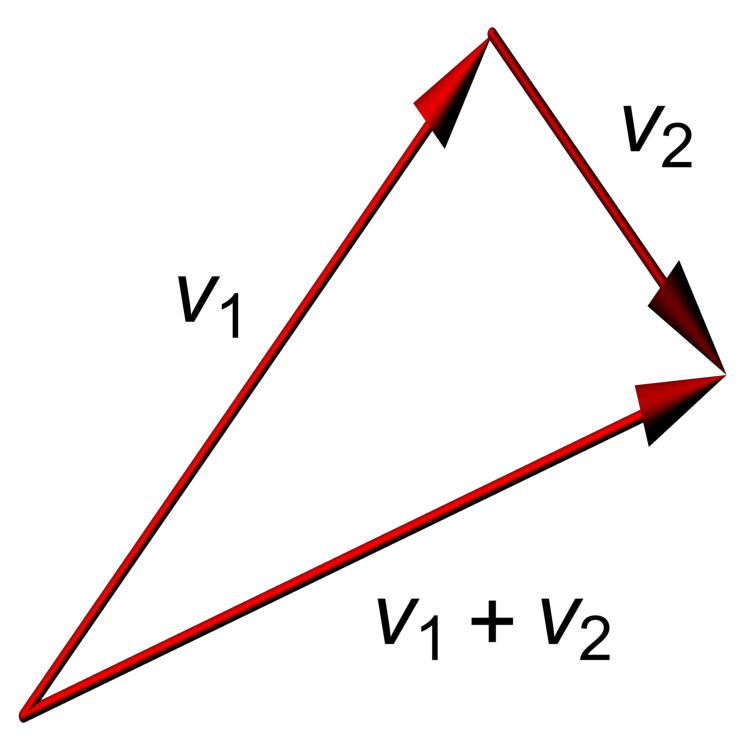
\includegraphics[width=0.45\textwidth]{vectorAddition}
  \caption{Illustration of vector addition in two dimensions.}
  \label{fig:vectorAddition}
\end{figure}
An essential part in designing a solution for the above problem is to decide, which representation to use internally for vectors. The Cartesian representation of a vector is as a tuple of real values $(x,y)$, where $x$ and $y$ are real values, and where we can imagine that the tail of the vector is in the origin, and its tip is at the coordinate $(x,y)$. For vectors on Cartesian form,
\begin{align}
  \vec v = (x,y),
\end{align}
the basic operations are defined as
\begin{align}
  \vec v_1 + \vec v_2 &= (x_1+x_2, y_1+y_2),
  \\a\vec v &= (a x,a x),
  \\\text{dir}(\vec v) &= \tan\frac{y}{x},\, x\neq 0,
  \\\text{len}(\vec v) &= \sqrt{x^2+y^2},
\end{align}
where $x_i$ and $y_i$ are the elements of vector $\vec v_i$, $a$ is a scalar, and $\text{dir}$ and $\text{len}$ are the direction and length functions. The polar representation of vectors is also a tuple of real values $(\theta, l)$, where $\theta$ and $l$ are the vector's direction and length. This representation is closely tied to the definition of a vector, and with the constraint that $0 \leq \theta < 2\pi$ and $0 \leq l$. This representation reminds us that vectors do not have a position. For vectors on polar form,
\begin{align}
  \vec v &= (\theta,l),
\end{align}
their basic operations are defined as
\begin{align}
  x(\theta,l) &= l\cos(\theta),
  \\y(\theta,l) &= l\sin(\theta),
  \\\vec v_1 + \vec v_2 &= (x(\theta_1,l_1)+x(\theta_2,l_2), y(\theta_1,l_1)+y(\theta_2,l_2))
  \\a\vec v &= (\theta,a l),
\end{align}
where $\theta_i$ and $l_i$ are the elements of vector $\vec v_i$, $a$ is a scalar, and $\text{x}$ and $\text{y}$ are the Cartesian coordinate functions.

So far in our analysis, we have realized that:
\begin{itemize}
\item both the Cartesian and polar representation uses a pair of reals to represent the vector, 
\item both require functions to calculate the elements of the other representation, 
\item the polar representation is invalid for negative lengths, and
\item the addition operator under the polar representation is also more complicated and essentially requires access to the Cartesian representation.
\end{itemize}
 

The first step in shaping our solution is to decide on file structure: For conceptual separation, we choose to use a library and an application file. F\# wants files to define namespaces or modules, so we choose the library to be a \lstinline{Geometry} module, which implements the vector class to be called \lstinline{vector}. Further, when creating vector objects, we would like to give the application program the ability to choose either Cartesian or polar form. This is can be done using \idx{discriminated unions}. Discriminated unions allow us to tag values of possibly identical form, but they also implied longer programs. Thus, we will also provide an additional constructor on implicit Cartesian form, since this is the most common representation.

A key point, when defining libraries, is to consider their interface with the application program. Hence, our second step is to write an application using the yet to be written library in order to get a feel for how such an interface could be. This is demonstrated in the application program \Cref{vectorAppCode}.
%
\fsCode{vectorApp}{vectorAppCode}{An application using the library in \Cref{vector}.}{}
%
The application of the vector class seems natural, makes use of the optional discriminated unions, and uses the infix operators \lexeme{+} and \lexeme{*} in a manner close to standard arithmetic, and interacts smoothly with the \lstinline{printf} family. Thus, we have further sketched requirements to the library with the emphasis on application.

After a couple of trials, our library implementation has ended up as shown in \Cref{vector}.
%
\fsImplementation{vector}{vector}{A library serving the application in \Cref{vectorApp}.}{}
%
Realizations achieved during writing this code are: Firstly, in order to implement a vector class using discriminated unions, we had to introduce a constructor with helper variables \lstinline{_x}, \lstinline{_y}, etc. The consequence is that the Cartesian and polar representation is evaluated once and only once every time an object is created. Unfortunately, discriminated unions do not implement guards on subsets, so we still have to cast an exception, when the application attempts to create an object with a negative length. Secondly, for the \lstinline{ToString} override we have implemented static members for typesetting vectors since it seems more appropriate that all vectors should be typeset identically. Changing typesetting thus respect dynamic scope.

The output of our combined library and application is shown in \Cref{vectorApp}.
%
\fsOutput{vectorApp}{Compiling and running the code from \Cref{vector} and~\ref{vectorAppCode}.}
%
The output is as expected and for the vector class, our solution seems to be a good compromise between versatility and syntactical bloating.

%%% Local Variables:
%%% TeX-master: "fsharpNotes"
%%% End:

